\section{Background}

We first briefly review speculative decoding~\citep{leviathan2023fast}, a critical technique that accelerates inference of a large target LLM $p(\cdot|\vx)$ with token proposals from a small draft model $q_\vtheta(\cdot|\vx)$. 
$\vx$ denotes the concatenation of the input prompt and already generated tokens. %
The two distributions are both auto-regressive. 
We emphasize the parameters $\vtheta$ of the draft model because we usually need to tailor them according to the target LLM for more substantial acceleration. 

Speculative decoding uses a (small) draft model to propose $k$ tokens ${\vy} \triangleq \{ y_i\}_{i=1}^k \sim q_\vtheta(\cdot | \vx)$, and let the target LLM estimate the $k+1$ probabilities, $\{p({y}|\vx, {\vy}_{<i})\}_{i=1}^{k+1}$\footnote{${\vy}_{<i}$ refers to $\{ y_j\}_{j=1}^{i-1}$.}, in parallel. %
With $i$ rising from $1$ to $k$, speculative decoding accepts the proposal ${y}_i$ if $u \leq  p(y_i|\vx, {\vy}_{<i}) / q_\vtheta({y}_i|\vx, {\vy}_{<i})$ where $u \sim U[0,1]$; otherwise exits. 
Let $a$ denote the number of accepted tokens, which takes values in $\{0,\dots, k\}$. %
We can sample an additional token ${y}_{a+1}$ from the following distribution 
\begin{equation}
p'(y) =
    \begin{cases}
      p(y|\vx, {\vy}_{<a+1}) & \text{if $a = k$}\\
      \mathrm{norm}(\max(0, p(y|\vx, {\vy}_{<a+1}) - q_\vtheta(y|\vx, {\vy}_{<a+1}))) & \text{otherwise}
    \end{cases}       
\end{equation}
where $\mathrm{norm}(\cdot)$ makes the probabilities over the vocabulary sum to $1$. 

Prior work has shown that the resulting samples $\tilde{\vy} \triangleq \{{y}_1, \dots, y_{a+1}\}$ strictly follow the distribution of the target LLM $p(\cdot|\vx)$~\citep{leviathan2023fast}. 
We concatenate $\tilde{\vy}$ to $\vx$ and repeat the above process until meeting ⟨EOS⟩. 
Each run of the target LLM generates $a+1$ tokens with $a\geq0$. This ensures that at least one new token is generated even in the worst case. 
The generation process can be significantly accelerated if the draft LLM better approximates the target one, particularly $a$ is larger for each target LLM run.


\textbf{Expected acceptance rate \& speedup.} 
The acceptance rate, denoted as \(\alpha\), serves as a measure of how closely the draft model approximates the target model. It is defined as the expected probability that speculative decoding will accept a proposal token given the prompt \(y_i \sim q_\vtheta(y_i|\vx, {\vy}_{<i})\). This rate directly influences the expected length ($\E(|\tilde{\vy}|)$) of \(\tilde{\vy}\) for each target LLM run and the speedup brought by speculative decoding. 

Assuming that the \(k + 1\) simultaneous evaluations of the target LLM \(p\) take roughly the same amount of time as generating a single token in parallel, %
let \(c\) be the time ratio for a single run between \(q_\vtheta\) and \(p\). The expected generation length of a single target LLM run and the speedup in the total wall time due to speculative decoding is represented as~\citep{leviathan2023fast}:
\begin{equation}
\label{eq:gen_len}
    \E(|\tilde{\vy}|) = \frac{1 - \alpha^{k+1}}{1-\alpha},\quad \E(speedup)=\frac{1-\alpha^{k+1}}{(1-\alpha)(kc+1)}.
\end{equation}
We depict the speedup for varying values of \(\alpha\) in Figure~\ref{fig:analysis-alphas}, which demonstrates the importance of $\alpha$ in affecting the speedup.

\begin{figure}[h]       
    \centering
    \label{fig:analysis-alphas}
    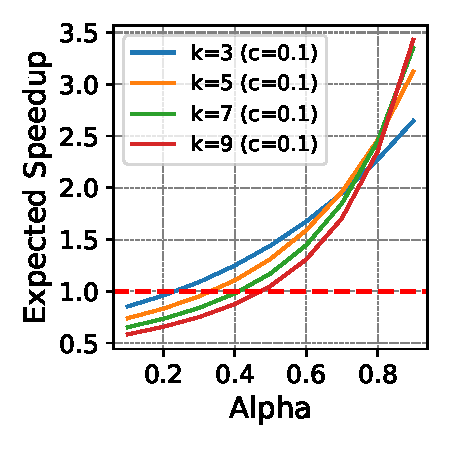
\includegraphics[width=0.25\linewidth]{figures/analysis_k.pdf}
    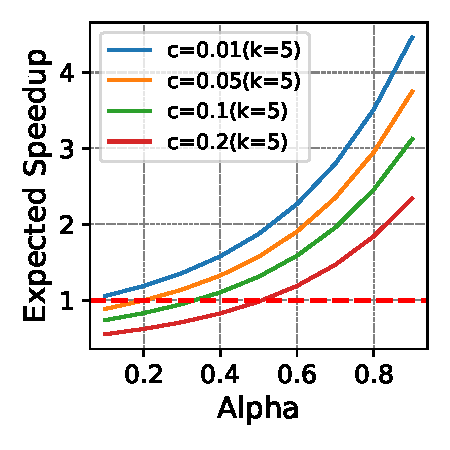
\includegraphics[width=0.25\linewidth]{figures/analysis_c.pdf}
    \caption{Speculative decoding speedups for varying values of \(\alpha\) in Figure~\ref{fig:analysis-alphas}. For smaller \(\alpha\) values, speculative decoding may even degrade performance (indicated by a speedup \(<1\)), particularly when the draft model is sizeable. Furthermore, the relationship between speedup and \(\alpha\) is superlinear; doubling the acceptance rate can yield a speedup exceeding 2$\times$.}
\end{figure}



{\bf Observation.} Interestingly, we can actually enhance \(\alpha\) based on a key observation: the speculative decoding process inherently identifies the inaccuracies of the small draft LLM and offers correct solutions for these inaccuracies. This essentially means that we receive valuable insights on the areas and strategies to refine the draft model at no additional cost. 
Viewed through the lens of online learning, we can effortlessly accumulate a set of input-output pairs, denoted as \( ([\vx, \vy_{<a+1}], p(y|\vx, {\vy}_{<a+1})) \), that have yet to be assimilated by the draft LLM, paving the way for its subsequent optimization. Given the reduced size of the draft model (for instance, it may be over $20\times$ smaller than the target model), its tuning is not only efficient but also viable for real-time online adjustments. 
Prior work~\citep{leviathan2023fast,miao2023specinfer} has primarily approached speculative decoding in an offline manner, meaning the draft model remains static during online deployment. We next develop online speculative decoding to bridge this gap.







\section{Online Speculative Decoding}
\label{sec:methodology}
We propose the online speculative decoding approach to update the draft model dynamically for more effective suggestions. 
We frame the learning problem based on the aforementioned auxiliary information as online knowledge distillation, where the teacher and student models correspond to the target and draft LLMs in speculative decoding, respectively. 
We elaborate on the details below. 


\subsection{Knowledge Distillation for Speculative Decoding}
\label{sec:knowledge-distill}
Knowledge distillation is a general framework to align the predictive distribution of a small model (i.e., student model) 
with that of a larger one (i.e., teacher model).
Prior research has utilized knowledge distillation to compress neural networks, resulting in decreased inference costs and memory requirements. 
We posit that knowledge distillation is highly effective for speculative decoding. 
In this approach, the draft model acts as the student and the target model serves as the teacher. 
During speculative decoding, we possess complete information on both the proposed and verified probabilities of each token. 
This information helps to construct objectives for distilling the draft model, aligning its output distributions with those of the target model 
and thereby improving the token acceptance rate of the draft model.
The distillation loss generally takes the form of:
\begin{equation}
    \label{eq:distill}
    \small
    \begin{aligned}
        \ell(\vtheta) &= \frac{1}{n_B}\sum_{\vx^{(i)} \in \mathcal{B}} \ell(\vx^{(i)}, \vtheta), \quad \ell(\vx, \vtheta) =  D ({p(\cdot|\vx)} \Vert {q_\vtheta(\cdot|\vx)} ),%
    \end{aligned}
\end{equation}
where $\mathcal{B} = \{\vx^{(i)}\}_{i=1}^{n_B}$ denotes a batch of inputs and $D$ denotes some distance measure. 

\textbf{Distance measure.} 
In the case of auto-regressive models, the prediction distribution is categorical at each token. 
Often, we can augment the predicted logits with a tunable temperature $\tau$ for softmax transformation. 
We then use the popular forward KL and reverse KL (RKL), as well as their mixture (i.e., the JSD divergence) 
to instantiate $D$~\citep{agarwal2023gkd,gu2023knowledge}:
\begin{equation}
    \small
    \begin{aligned}
        &\ell_{KL}(\vx, \vtheta) = \KL( {p(\cdot|\vx)}\Vert {q_\vtheta(\cdot|\vx)}), \\
        &\ell_{RKL}(\vx, \vtheta) = \KL({q_\vtheta(\cdot|\vx)} \Vert {p(\cdot|\vx)}), \\
        &\ell_{{JSD}[\beta]} (\vx, \vtheta) = \beta \KL \left({p(\cdot|\vx)} \big\Vert {p}^\beta_\vtheta(\cdot|\vx)\right)+ (1-\beta) \KL \left({q_\vtheta(\cdot|\vx)} \big\Vert {p}^\beta_\vtheta(\cdot|\vx)\right),
    \end{aligned}
\end{equation}
where ${p}^\beta_\vtheta(\cdot|\vx) \triangleq \beta{p(\cdot|\vx)} + (1-\beta){q_\vtheta(\cdot|\vx)}$. 
These objectives diverge from the conventionally used label-based fine-tuning objectives in speculative decoding, 
as highlighted in~\citep{miao2023specinfer, leviathan2023fast}. As shown in Section~\ref{sec:offline-eval},
objectives based on the KL divergence prove to be more effective. This is because distributions 
convey richer information than mere labels, thereby enhancing their capability to guide the student model~\citep{hinton2015distilling}. 
Additionally, these objectives enhance convergence rates~\citep{he2022knowledge} and bolster calibration. 
The reverse KL is highlighted for its mode-seeking behavior, offering unique advantages~\citep{gu2023knowledge}. 
In our study, and in alignment with previous research~\citep{agarwal2023gkd}, we empirically determine that the optimal 
distance measure can vary depending on the tasks and the relative capacities of the teacher and student models (see \S\ref{sec:offline-eval}).


\textbf{Sampling and gradient estimation.}
Estimating the above objectives involves the expectation over $q_\vtheta(\cdot|\vx)$ or $p(\cdot|\vx)$, which should be expanded recursively. 
Once the recursion depth exceeds $1$, we can not analytically compute $\KL$ but hinge on Monte Carlo approximation. 
When sampling from $q_\vtheta(\cdot|\vx)$, we should differentiate through the sampling process for unbiased gradient estimation. 
However, this leads to policy gradient-style estimators and should rely on elaborate policies such as reward hacking and single-step regularization to reduce gradient variance and stabilize training~\citep{gu2023knowledge}. 

In comparison, a more straightforward approach is to omit the differentiation through the sampling process~\citep{agarwal2023gkd}, where the sample $\vy$ is directly plugged into the objective:
\begin{equation}
\label{eq:offline}
    \small
    \ell(\vx, \vtheta) \approx
 \sum_{j =1}^{|\vy|+1} D({p(y|\vx, \vy_{<j})} \Vert {q_\vtheta(y|\vx, \vy_{<j})} ).
\end{equation}
This way, various distance measures can be readily applied.
Besides, the sampling becomes disentangled from the distance measure. i.e., we sample $\vy$ from an arbitrary mixture of ${p}(\cdot|\vx)$ and ${q}_\theta(\cdot|\vx)$ but use KL, RKL or JSD for estimating the distribution mis-alignment. 

Intuitively, the samples from the teacher model are usually coherent, which may raise difficulties in fitting the small student model, while samples from the student model may be less structured or even meaningless. 
A workaround strategy is to trade off between them via mixed sampling~\citep{gu2023knowledge}, i.e., $y_j \sim \beta{p(\cdot|\vx, \vy_{<j})} + (1-\beta) q_\vtheta(\cdot|\vx, \vy_{<j})$. 







\subsection{Online Knowledge Distillation}
This section expands the application of knowledge distillation for speculative decoding in online environments. 
The approach enables improving the performance of draft model using results from speculative decoding, 
thus dynamically adapting to the query distribution and improving token acceptance rate. 
We also discuss the trade-off of our approach when integrating LLM serving systems.


\subsubsection{Algorithm}
\begin{algorithm}[t] 
\caption{Online Speculative Decoding.} 
\label{algo:1}
\small
\begin{algorithmic}[1]
\STATE {\bfseries Input:} 
Target LLM $p(\cdot|\vx)$, draft LLM $q_\vtheta(\cdot|\vx)$, warmup dataset $\mathcal{D}$, online data stream $\mathcal{S}$, guess number $k$, temporary buffer $\mathcal{R}$, replay buffer $\mathcal{Q}$, update interval for the draft model $I$.
\STATE{Pre-train $q_\vtheta$ to approximate $p$ with data from $\mathcal{D}$ by minimizing $\ell(\vx, \vtheta)$ using \cref{eq:offline};}
\STATE{$i \leftarrow 0$;}
\STATE{$\mathcal{Q} \leftarrow []$;}
\STATE{$cur\_len = |\vx|$ // Total sequence length, including prompt length and tokens generated so far.}
\WHILE{True}
    \STATE{$\mathcal{R} \leftarrow []$ // List of ($error\_index$, target logits at $error\_index$) pairs for a single request.}
    \STATE{$\vx \sim \mathcal{S}$, $i \leftarrow i + 1$;}
    \WHILE{⟨EOS⟩ not in $\vx$}
    \STATE{${\vy} = \{{y}_1,...,{y}_k\} \sim q_\vtheta(\cdot|\vx)$;}
    \STATE{Estimate $\{p({y}|\vx, {\vy}_{<i})\}_{i=1}^{k+1}$ in parallel;}
    \STATE{Determine number of accepted tokens $a$ and sample one more token, yielding $\vy=\{{y}_1, \dots, y_{a+1}\}$;} 
    \STATE{$cur\_len \leftarrow cur\_len + a + 1$;}
    \STATE{$error\_index \leftarrow cur\_len$;}
    \STATE{Append $(error\_index, p(y|\vx, {\vy}_{<a+1}))$ to $\mathcal{R}$;}
    \STATE{$\vx \leftarrow [\vx, {\vy}_{<a+2}]$;}
    \ENDWHILE
    \STATE{Append $(\vx, \mathcal{R})$ to $\mathcal{Q}$;}
    \IF{$i\;\mathrm{mod}\;I = 0$}
    \STATE{Update $q_\vtheta$ on $\mathcal{Q}$ to minimize $\ell(\vx, \vtheta)$ analytically;}
    \STATE{$\mathcal{Q} \leftarrow []$;}
    \ENDIF
\ENDWHILE
\end{algorithmic}
\end{algorithm}

We depict our online speculative decoding algorithm (\tool) in \cref{algo:1}.
\tool begins by training the draft model using the warmup dataset (Line 2). 
The serving system then continuously handles incoming requests (as described in Lines 6 to 23).
For each request, it uses standard speculative decoding (Lines 10-11) to generate responses until the ⟨EOS⟩ token. 
Concurrently, \tool tracks the token index ($error\_index$) and target logits where the draft model proposes the wrong tokens (Line 15). 
Leveraging tracked information, \tool updates the draft model every $I$ iteration, with $I$ being a dynamically adjustable parameter.
\tool updates the draft model with different loss functions (Line 20) as described in Section~\ref{sec:knowledge-distill}.
The choice of loss function depends on the specific (draft, target) model pairs and the corresponding input data. 

{\bf Discussion.} 
\tool utilizes a replay buffer, $\mathcal{Q}$, to capture all pertinent information for updating the draft model. 
Various eviction policies can be employed to maintain a compact size for $\mathcal{Q}$. 
For example, one could opt to retain only the most informative pairs or the most recent entries. 
Similarly, users have the option to retain data in $\mathcal{Q}$
even after utilizing it to update the model multiple times.
Determining the optimal eviction/retention strategy is a subject for future exploration. 
In the current study, we refrain from evicting any pairs and release $\mathcal{Q}$ after each model update.
Furthermore, $I$ is a dynamic parameter. Depending on the system load and the rate at which the query
distribution changes, users can adjust $I$ accordingly.
For example, we can perform a gradient update opportunistically only when the service traffic is not on spike (i.e., spare flops are available).
Overall, \tool continuously improves the draft model's approximation (indicated by increased token acceptance rate $\alpha$) 
by learning from the target model during the serving phase. We next demonstrate how the enhanced acceptance rate directly 
contributes to a reduction in request latency.





\subsubsection{Latency \& Flops Analysis} 
\label{sec:analysis}
{\bf Latency.} As detailed in  Appendix~\ref{appendix:latency-analysis}, compared with standard speculative decoding, 
the expected speedup for online speculative decoding is  \( \frac{1+\alpha_2+\alpha_2^2+...+\alpha_2^{k}}{1+\alpha_1+\alpha_1^2+...+\alpha_1^k}\).
Based on the data from our experiment (refer to Table~\ref{tab:apha}), when compared to standard speculative decoding, 
we expect a speedup %
improvement for Vicuna-7B (LLaMA-160M as the draft model) by factors of \(2.42\times\), \(1.43\times\), \(1.64\times\), and \(1.22\times\). Similarly, for Flan-T5-XL 3B (T5-small 80M as the draft model), the speedup enhancements are \(3.06\times\), \(1.76\times\), \(2.72\times\), and \(1.55\times\) across the four evaluated datasets. %

{\bf FLOPs.}
(1) The FLOPs required to update the draft model are significantly fewer than those needed for inference on a large model. 
As elaborated in Appendix~\ref{appendix:flops}, for the two evaluated model pairs, 
the FLOPs ratio between the target model and the draft model is 18.75 for the pair (LLaMA-160M, Vicuna7B), and 12.6 for the pair (T5-small 80M, Flan-T5-XL 3B). 
(2) In practical systems, the FLOPs required for inference are significantly below the machine's capacity.
The Appendix~\ref{appendix:flops} provides an analysis of Arena chatbot traces where the cluster's computational utilization is under 1 percent. %
Given the above two observations, it becomes evident that the FLOPs spent on inference and updating the draft model are relatively 
insignificant when juxtaposed with the FLOPs consumed while operating the target model and the cluster's total FLOPs.







